The following chapter of this thesis will offer a comprehensive exploration of the platform that provides the data for this study. These sections will explore the available options and the process used to select the final dataset. Additionally, they will present a detailed explanation of the dataset itself and describe the natural language processing (NLP) techniques employed in the analysis, ensuring an understanding of its structure, content, and the methods used to extract insights.

\section{Dataset}
\label{subsec:datasets}
Kaggle was selected as the source for the dataset due to several practical considerations. Kaggle offers a wide array of pre-processed and well-documented datasets that are immediately usable, which significantly reduces the preparation workload.
Furthermore, many platforms that provide access to raw data, especially social media platforms, require the use of APIs that are often not free. In contrast, Kaggle provides free access to various datasets, including those related to climate change and sentiment analysis, making it an economically reasonable option. Thus, choosing Kaggle was a strategic decision to maximize efficiency, manage resources effectively, and follow the academic and financial limitations of the thesis project.

\subsection{Kaggle}
Kaggle has rapidly become a crucial platform in the data science community, particularly valued in academic and research settings for its wide range of tools that promote innovation, collaboration, and education in data-driven disciplines.

\subsection{Options and Selection}
In the upcoming sections, we will explore five distinct datasets, evaluating their advantages and disadvantages to determine their suitability for this research. The detailed analysis will guide the decision-making process, leading to the selection of the most appropriate dataset that effectively supports the objectives of the thesis. This careful selection ensures that the research is built on a solid foundation, improving the reliability and validity of the findings.

\subsubsection{Climate Change Tweets}

The dataset Climate Change Tweets \cite{ClimateChangeTweets} consists of a single CSV file, sized at 4.94 MB, containing the top daily tweets from X\footnote{Twitter was rebranded to \emph{X} on July 22, 2023. Despite the rebranding of Twitter to "X", the posts on the platform are still referred to as "tweets."} that include the keyword "climate change." The data covers the time period from January 1, 2022, to July 19, 2022, and was collected using the \emph{Scweet} tool. It includes 9,050 entries across 11 columns, with the most important columns being UserName, Timestamp, Text, Likes, Retweets, and Comments. Figure \ref{fig:ds_1_activity} presents the Activity Overview of the dataset as provided by Kaggle. It indicates that the dataset is still actively reviewed and downloaded, demonstrating ongoing interest and engagement with the data. 

\begin{figure}[h]
    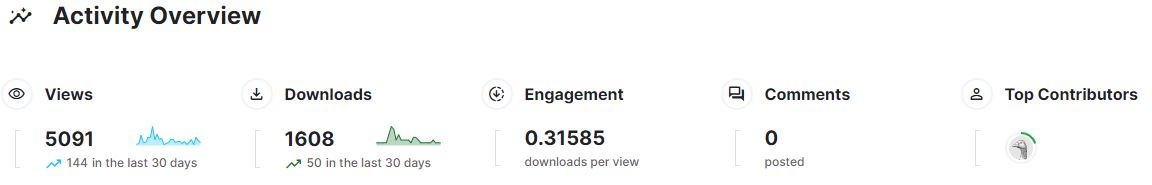
\includegraphics[width=\textwidth]{images/dataset/ds_1_activity.JPG}
    \caption{Activity Overview of the \emph{Climate Change Tweets} Dataset\protect\footnotemark}
    \label{fig:ds_1_activity}
\end{figure}
\footnotetext{Checked on May 9, 2024}

\paragraph{Dataset Advantages}
\begin{itemize}
    \item The dataset includes the text of each tweet along with its timestamp, providing a clear timeline of discussions.
    \item Metadata such as Likes, Retweets, and the number of comments are available, offering insights into the engagement each tweet received.
    \item The data is relatively recent, increasing its relevance to current studies on public opinion regarding climate change.
\end{itemize}

\paragraph{Dataset Disadvantages}
\begin{itemize}
    \item No sentiment scores are provided, requiring additional processing to analyze the sentiment of the tweets.
    \item The dataset covers only a seven-month period, limiting the ability to observe long-term trends or seasonal variations in the discussion of climate change.
    \item Accompanying the dataset is a single Jupyter notebook that contains minimal code unrelated to the dataset, offering little in terms of analysis or insights.
    \item There have been no updates to the dataset for two years, raising concerns about its currency and ongoing relevance.
\end{itemize}

\subsubsection{Climate Sentiment in Twitter}
The dataset Climate sentiment in twitter \cite{ClimateSentimentInTwitter} contains a single CSV file sized at 132.38 kB, containing 396 tweets with 14 columns, sourced from X between January 1, 2020, to December 24, 2020. It was gathered using the X API via the Tweepy library. Figure \ref{fig:ds_2_activity} shows that there is still user engagment, but not as active as for the previous dataset.

Key columns in the dataset include date, retweets, likes, text, location, and whether the user is verified. These columns offer valuable metadata about the timing, geographical context, and user engagement with each tweet.

\begin{figure}[h]
    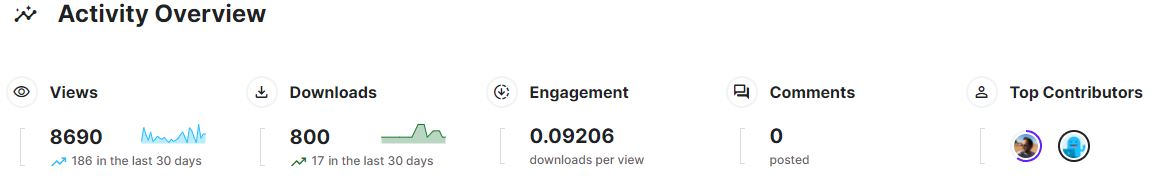
\includegraphics[width=\textwidth]{images/dataset/ds_2_activity.JPG}
    \caption{Activity Overview of the \emph{Climate sentiment in twitter} Dataset\protect\footnotemark}
    \label{fig:ds_2_activity}
\end{figure}
\footnotetext{Checked on May 10, 2024}

\paragraph{Dataset Advantages}
\begin{itemize}
    \item The dataset provides comprehensive metadata, particularly concerning time, location, and user interaction, which are crucial for detailed analyses.
    \item The methodology for data collection is documented, allowing for the potential expansion of the dataset using the specified Twitter API filters.
\end{itemize}

\paragraph{Dataset Disadvantages}
\begin{itemize}
    \item The overall description of the dataset is lacking, making it difficult to understand all aspects of the data without deeper investigation.
    \item It does not include sentiment scores, which would require additional processing to analyze the sentiment of the tweets
    \item The dataset is relatively small, covering only one year with an average of approximately 1.1 tweets per day covering only 1 year, which limits the scope of analysis.
    \item The data are somewhat outdated and not being updated anymore, which could affect the relevance and usefulness of the findings for current applications.
\end{itemize}

\subsubsection{Twitter Climate Change Sentiment Dataset}
The dataset Twitter Climate Change Sentiment Dataset \cite{TwitterClimateChangeSentimentDataset} provides a single CSV file of 6.57 MB, containing 43,943 tweets that have been annotated to reflect various sentiments toward climate change. These tweets are dated from April 27, 2015, to February 21, 2018, which was supported by a grant from the Canada Foundation for Innovation JELF, awarded to Chris Bauch at the University of Waterloo. The dataset includes three main columns: Sentiment, Message, and TweetID. The sentiment classes are detailed as follows:
\begin{itemize}
    \item \textbf{-1 (Anti):} The tweet expresses disbelief in man-made climate change.
    \item \textbf{ 0 (Neutral):} The tweet neither supports nor denies man-made climate change.
    \item \textbf{ 1 (Pro):} The tweet supports the belief in man-made climate change.
    \item \textbf{ 2 (News):} The tweet relays factual news about climate change.
\end{itemize}
Each tweet in the dataset was independently reviewed by three annotators for sentiment classification. A tweet was included in the final dataset only if there was unanimous agreement among all three reviewers regarding its sentiment class. The data were gathered using the X API within the specified date range. The methodology guarantee a comprehensive representation of public sentiment over the observed period.
Moreover, the dataset comes with detailed documentation that explains how the data was collected and labeled. Also, it includes nine notebooks created by different authors, filled with a lot of code to help with analyzing the data. Furthermore, this dataset has the most user attention of all datasets presented. Its activity overview can be found in figure \ref{fig:ds_3_activity}

\paragraph{Dataset Advantages}
\begin{itemize}
    \item The dataset is well-documented, providing clear insights into the data gathering and annotation processes.
    \item It is the largest dataset of its type currently developed, increasing its value for extensive research studies.
    \item The quality of the data is notably high, making it a reliable source for detailed analysis.
    \item High amount of existing code examples offer valuable resources for reuse and customizations, supporting further research and development. 
\end{itemize}
\paragraph{Dataset Disadvantages}
\begin{itemize}
    \item The dataset includes only 43,943 tweets, a modest number given the nearly three-year  timeframe of data collection, potentially limiting the scope of analysis.
    \item The data, covering dates up to early 2018, may not reflect current sentiments or recent developments in climate change discourse.
    \item There is no detailed explanation regarding the criteria used for selecting tweets for annotation, which might affect the dataset's applicability for certain research questions.
\end{itemize}

\begin{figure}[h]
    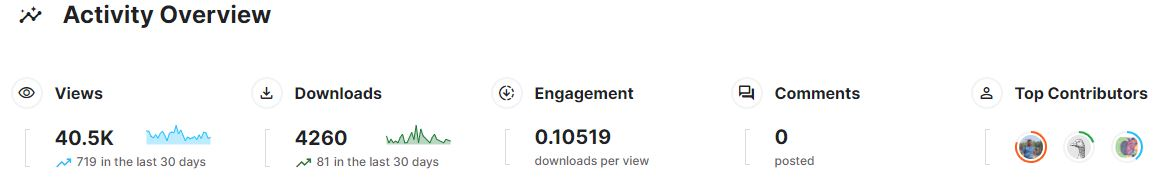
\includegraphics[width=\textwidth]{images/dataset/ds_3_activity.JPG}
    \caption{Activity Overview of the \emph{Twitter Climate Change Sentiment Dataset} Dataset\protect\footnotemark}
    \label{fig:ds_3_activity}
\end{figure}
\footnotetext{Checked on May 10, 2024}

\subsubsection{Social Media Sentiment and Climate Change}
The dataset Social Media Sentiment and Climate Change \cite{SocialMediaSentimentAndClimateChange} consists of six CSV files, with a combined size of 83.85 MB. The primary file in this dataset is the \emph{nltk\_split.csv} file. It includes important details such as the text of the posts, engagement metrics (favorite and retweet counts), the timestamp of posting, location coordinates, and an already calculated score for each post. Figure \ref{fig:ds_4_activity} shows its popularity.

\paragraph{Dataset Advantages}
\begin{itemize}
    \item Contains 164k posts.
    \item Provides a clear description on its Kaggle page.
    \item Covers about 20 months of data, from September 21, 2017, to May 19, 2019.
    \item Scores for posts are pre-calculated.
    \item Includes additional metadata for each post.
\end{itemize}

\paragraph{Dataset Disadvantages}
\begin{itemize}
    \item The methodology for score calculation is unknown.
    \item The latest entries are from mid-2019, making it around five years old.
    \item The specific social media platforms used for data collection are not identified.
    \item There appears to be redundancy among the data files.
    \item It is unclear whether "post" refers only to original content or also includes comments.
    \item There are no provided code examples to facilitate data analysis.
\end{itemize}

\begin{figure}[h]
    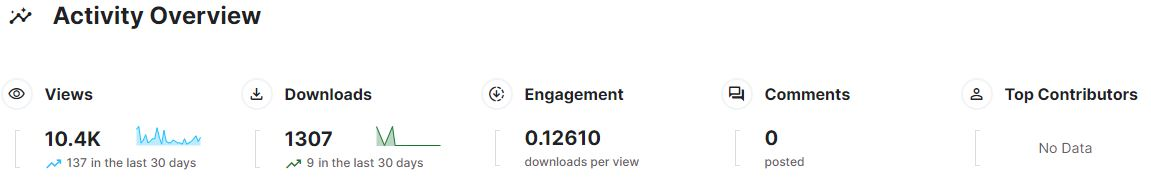
\includegraphics[width=\textwidth]{images/dataset/ds_4_activity.JPG}
    \caption{Activity Overview of the \emph{Social Media Sentiment and Climate Change} Dataset\protect\footnotemark}
    \label{fig:ds_4_activity}
\end{figure}
\footnotetext{Checked on May 11, 2024}

\subsubsection{The Reddit Climate Change Dataset}
The dataset The Reddit Climate Change Dataset \cite{TheRedditClimateChangeDataset} contains two CSV files obtained through \emph{SocialGrep Exports}, which collects all hits on \emph{climate} and \emph{change} that appear in the same comment (they don't necessarily need to appear as bigram): one file contains 620k posts and the other 4.6M comments, covering an extensive data range from January 1, 2010, to August 31, 2022, totaling about 12.5 years. The posts file includes 12 columns, with key columns being subreddit.name, created\_utc, and selftext. This file captures the important details of each post within the subreddit context. The comments file features 12 columns, notably created\_utc, body, and sentiment. This file provides insights into user interactions and sentiment across various discussions. Additionally, several code examples are provided to simplify data handling and analysis.
 
\begin{description}
    \item[SocialGrep Exports] is a feature offered by the SocialGrep tool \cite{SocialGrepExports}, which is designed to export and analyze data from social media platforms, notably Reddit. This feature enables users to download large datasets that include metrics such as post counts, engagement data, and sentiment analysis, all of which are useful for deep insights into social media trends and user behavior. The tool, SocialGrep, is owned and developed by Lexyr Inc., a company specializing in data analytics and extraction services. This makes SocialGrep an elemental part of Lexyr Inc.'s suite of tools that assist researchers, marketers, and analysts in using the power of big data from social media for various applications, from market research to academic studies.
\end{description}

\paragraph{Dataset Advantages}
\begin{itemize}
    \item Covers over 5 million posts and comments, offering a vast pool of social media interactions for analysis.
    \item Covers a considerable time period, including recent data up to August 2022.
    \item Pre-calculated scores for posts and comments are included, adding a layer of analysis readiness.
    \item Clear documentation of data sources improves the dataset's reliability.
    \item Availability of code examples benefits immediate data manipulation and analysis.
\end{itemize}

\paragraph{Dataset Disadvantages}
\begin{itemize}
    \item The description on Kaggle is not detailed, leaving several questions unanswered.
    \item A significant number of posts are inaccessible due to various restrictions like paywalls or provider limitations.
    \item Lack of clarity on how the scores for posts and comments were calculated.
    \item Both files include a 'score' column. However, the exact significance and calculation method of these scores are not fully explained.
    \item The large size of the files (262 MB and 4.11 GB) demands considerable computing resources and efficient programming to manage without exceeding system memory limits.
    \item There is no established linkage between posts and their corresponding comments, which complicates integrated analysis of conversations.
\end{itemize}

Despite its large data size, this dataset shows the highest engagement among all Kaggle datasets presented, as illustrated in Figure \ref{fig:ds_5_activity}.

\begin{figure}[h]
    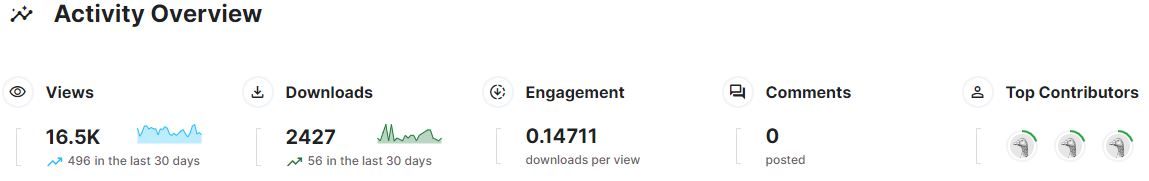
\includegraphics[width=\textwidth]{images/dataset/ds_5_activity.JPG}
    \caption{Activity Overview of the \emph{The Reddit Climate Change Dataset} Dataset\protect\footnotemark}
    \label{fig:ds_5_activity}
\end{figure}
\footnotetext{Checked on May 11, 2024}

\subsubsection{Final Dataset Selection}
\begin{table}[h!]
    \centering
    \begin{tabular}{c c c c c}
    \toprule
    \textbf{Dataset} & \makecell{\textbf{Number of} \\ \textbf{Comments}} & \makecell{\textbf{Level of} \\ \textbf{Documentation}} & \makecell{\textbf{Code} \\ \textbf{Availability}} & \makecell{\textbf{Sentiment} \\ \textbf{Availability}} \\
    \midrule
    \makecell{Climate Sentiment \\ in Twitter} & 396 & - & Yes & No \\
    \hline
    \makecell{Climate Change \\ Tweets} & 9,050 & - & No & No \\
    \hline
    \makecell{Twitter Climate \\ Sentiment Change \\ Dataset} & 43,943 & + & Yes & Yes \\
    \hline
    \makecell{Social Media \\ Sentiment and \\ Climate Change} & 164,000 & + & No & No \\
    \hline
    \makecell{The Reddit Climate \\ Change Dataset} & 4,600,698 & 0 & Yes & Yes \\
    \bottomrule
    \end{tabular}
    \caption{Datasets and their Key Properties for Dataset Selection}
    \label{table:datasets}
\end{table}

The dataset \emph{The Reddit Climate Change Dataset} is a great choice (see Table \ref{table:datasets} for a brief comparison) for studying how people feel about climate change because it covers a lot of ground and provides plenty of information. It covers a period of twelve years, which lets researchers see how opinions on climate change have changed due to major events, policy updates, and news coverage. With more than five million posts and comments, it covers a wide range of viewpoints, making sure that many different opinions are included.

The dataset also includes scores that hint at whether comments are positive, negative, or neutral towards climate change. These pre-calculated scores make it easier to quickly figure out the general mood in the data. Researchers can use these scores as a starting point to dive deeper into specific topics or time periods to understand how attitudes change.

Additionally, the dataset comes with some ready-to-use code, which makes it easier to start analyzing the data right away. This helps researchers focus on understanding the trends and patterns in how people talk about climate change, without getting pushed back by technical challenges. Overall, this dataset is very helpful for anyone looking to explore the complex ways people discuss and react to climate change over time.

\subsection{Reddit}
Reddit is one of the most popular social media platforms globally, especially noted for its appeal in English-speaking countries. Here, we provide a detailed breakdown of its demographics, language use, and popularity across different continents based on the latest data available.

\subsubsection{User Demographics and Global Reach}
\begin{description}
    \item[Geographical Distribution] As of 2023, the United States remains the dominant source of Reddit's traffic, accounting for approximately 47.89\% of all users. This high concentration highlights its significant impact on and usage by American audiences. Following the US, other significant traffic contributions come from:
    \begin{itemize}
        \item United Kingdom: 7.85\%
        \item Canada: 7.49\%
        \item Australia: 4.05\%
        \item Germany: 3.21\%
\end{itemize}
These figures underscore the platform's strong presence in predominantly English-speaking countries (Source: Alexa, 2023).

\item[User Age Group] The platform is particularly popular among younger demographics. Data from Statista (2023) indicate that:
\begin{itemize}
    \item 58\% of Reddit users are aged between 18 and 29 years.
    \item 29\% are aged between 30 and 49 years.
\end{itemize}
This demographic trend points to the platform's popularity among digital natives and younger internet users.

    \item[Gender Distribution] Approximately 70\% of Reddit users are male, which influences the type of content that is popular and the nature of discussions (Source: Statista, 2023).
\end{description}

\subsubsection{Language and Cultural Reach}
\begin{description}
    \item[Language Usage] While Reddit supports multilingual content, the predominant language of communication is English. This is reflected in the top countries by user base, all of which are primarily English-speaking nations. However, there are niche communities, known as subreddits, which meet specific languages and regional interests.
\end{description}

\subsubsection{Popularity Across Continents}
\begin{description}
    \item[North America and Europe] These regions represent the core user base of Reddit, with North America alone accounting for over half of all Reddit traffic. Europe, while having a diverse linguistic background, still contributes significantly to the user base due to the high English proficiency in countries like Germany, the UK, and the Nordic countries.
    \item[Asia and Other Regions] Reddit's presence in Asia is less pronounced, largely due to the prevalence of local social networks and language barriers. For instance, in China and South Korea, local platforms such as Weibo and Naver respectively, dominate the social media landscape. Reddit's market share in these regions is minimal.
    \item[Australia and Oceania] In Australia, Reddit enjoys considerable popularity, aligning with the global trend of English language dominance on the platform. The user engagement from this region is comparable to that of European countries.
\end{description}

\subsubsection{Conclusion}
These statistics provide a clear picture of Reddit's user base, highlighting its importance towards young, English-speaking populations primarily located in Western countries. This demographic and cultural profiling is crucial for understanding the context within which data from Reddit is generated and can be used in research to draw insights about Western, particularly American, public opinion and trends. Understanding these limitations is also vital for researchers using Reddit data to ensure that their findings are contextualized appropriately.

\section{Natural Language Processing Techniques}

\subsection{Sentiment Analysis and VADER}
\label{subsec:sentiment}
Sentiment analysis is a branch of natural language processing (NLP) that involves analyzing, understanding, and extracting opinions from text to determine the sentiment behind words. It is widely used to estimate public opinion, monitor brand and reputation, and understand customer emotions in text data.
\subsubsection{Toolkits for Sentiment Analysis}
There are several toolkits and libraries available for sentiment analysis, each offering unique features:
\begin{enumerate}
    \item \textbf{NLTK (Natural Language Toolkit):} This Python library is comprehensive for educational and research purposes, providing interfaces to over 50 corpora and lexical resources, including a built-in sentiment analysis module. It uses rule-based, lexicon-based methods for various NLP tasks \cite{BirdKleinLoper09}.
    \item \textbf{TextBlob:} Built on top of NLTK and Pattern, TextBlob is user-friendly for quick NLP tasks, offering a straightforward API for sentiment analysis. It provides a rule-based, lexicon-based API ideal for newcomers and intermediate users \cite{loria2018textblob}.
    \item \textbf{VADER (Valence Aware Dictionary and sEntiment Reasoner):} VADER is particularly tailored for social media analysis, employing a combination of qualitative and quantitative methods to determine sentiment. It excels in capturing the nuances of social media language, including emojis and slang. VADER uses lexicon-based methods with rule-based improvements \cite{hutto2014vader}.
    \item \textbf{spaCy:} Known for its speed and efficiency, spaCy supports sentiment analysis capabilities and is suitable for large-scale information extraction tasks, offering robust industrial-strength capabilities. spaCy is primarily automatic (machine learning), with support for rule-based extensions \cite{honnibal2017spacy}.
\end{enumerate}

\subsubsection{Approaches to Sentiment Analysis}
Sentiment analysis can be categorized into:
\begin{description}
    \item[Rule-Based Systems] Rule-based systems are tools which use specific grammar rules to figure out if words in a text are positive, negative, or neutral. They look closely at how sentences are built and pay attention to things like words that flip a meaning (like "not") or make it stronger or weaker. The great thing about these systems is that they're easy to understand. You can see how they work and even change the rules to suit your needs. This is really helpful when you need to explain why a piece of text was judged a certain way. However, these systems have some limitations. They can be hard to grow and adapt to new situations. It takes a lot of work to build and update them, especially when dealing with complicated texts or different languages and cultural settings. Also, they might not always get the sentiment right if the text has understated language keywords or cultural references that affect the meaning. This makes them less reliable in environments where language is constantly evolving or very diverse \cite{liu2012}.
    \item[Lexicon-Based Systems] Lexicon-based systems rely on a sentiment lexicon—a dictionary where each word is tagged with a predefined sentiment score. The overall sentiment of a text is calculated by summing the scores of the words present in the lexicon that appear in the text. This method is celebrated for its simplicity and efficiency, as it primarily involves dictionary lookups and arithmetic operations. However, its simplicity can also be a limitation. Lexicon-based systems typically do not account for the context surrounding words, which can lead to inaccuracies in texts where words may carry different sentiments depending on their usage. Moreover, these systems struggle with adaptability, often failing to recognize slang, idioms, or newly coined phrases that aren't included in the static lexicon. This makes lexicon-based sentiment analysis less reliable for texts that involve evolving language or colloquial expressions \cite{10.1162/COLI_a_00049}.
    \item[Automatic Systems] Automatic systems use machine learning algorithms to learn how to classify sentiment from large datasets of labeled text. These systems range from simpler models like logistic regression to more complex architectures such as deep learning models including Long Short-Term Memory (LSTM) networks or Convolutional Neural Networks (CNNs). One of the main advantages of automatic systems is their ability to understand complex language patterns and the context in which words are used, which significantly improves the accuracy of sentiment analysis across varied datasets. Additionally, these systems can adapt to new, unseen data if they are continuously trained, which is beneficial for applications involving dynamic language use. However, the dependency on large volumes of labeled training data makes these systems resource-intensive to develop. Furthermore, advanced models, particularly those based on deep learning, often lack interpretability, which can be problematic in settings where understanding the decision-making process behind sentiment analysis is essential \cite{yoonklim,pang2008opinion}.
    \item[Hybrid Systems] Hybrid systems represent an integration of rule-based, lexicon-based, and automatic methodologies, aiming to combine the strengths of each to optimize sentiment analysis. These systems might use machine learning models to analyze text structure and content, while rule-based adjustments are employed to refine the sentiment based on known linguistic cues. The flexibility and contextual relevance of hybrid systems are major advantages, as they allow for the integration of human insights through rules and tailored lexicons while using machine learning efficiencies. These systems often result in higher accuracy and robustness, particularly when dealing with specific linguistic or cultural distinctions. However, they can be complex to design and resource-intensive, requiring careful integration and significant computational power \cite{PORIA201650}.
\end{description}
These categories of sentiment analysis offer a spectrum of methodologies, each suited to different types of data and analysis needs. By understanding these distinctions, researchers and practitioners can better choose the approach that best fits their specific requirements for sentiment analysis.

\subsubsection{VADER and its Score}
VADER is specifically designed for sentiment analysis in social media contexts. Developed by Hutto and Gilbert (2014), VADER analyzes sentiments based on a lexicon of sentiment-related words and includes grammatical and syntactical rules to estimate textual sentiment. Its lexicon includes words that have been rated for their positive or negative sentiment valence based on common usage in social media environments. VADER is open-source, with its code and lexicon available on GitHub \url{https://github.com/cjhutto/vaderSentiment}, making it accessible for development and customization.

VADER outputs sentiment scores on a normalized, weighted composite scale. The compound score, which aggregates the cumulative sentiment of the text, ranges from -1 (extremely negative) to +1 (extremely positive). Scores are typically classified as follows:
\begin{itemize}
    \item \textbf{Positive sentiment:} compound score $\geq 0.05$
    \item \textbf{Neutral sentiment:} $-0.05 <$ compound score $< 0.05$
    \item \textbf{Negative sentiment:} compound score $\leq -0.05$
\end{itemize}
This scoring system allows for detailed interpretation of sentiment in text, particularly useful in dynamic and informal communication like social media posts. While VADER is highly effective for social media corpora, its performance can vary on more formal content or where context extends beyond the scope of its lexicon. Additionally, VADER may not always accurately interpret sarcasm, complex metaphors, or understated uses of language that may not directly trigger lexical keywords identified in its dictionary.

This detailed overview of sentiment analysis, particularly focusing on VADER, provides researchers and specialists with the necessary understanding to apply these methods effectively in different scenarios, especially where social media text analysis is required.

\subsection{Named Entity Recognition}
Named Entity Recognition (NER) is a process in natural language processing (NLP) where a computer reads a piece of text and highlights important names like people, companies, or places. This technology is crucial for understanding and organizing large amounts of data, as it helps convert unstructured text into structured data, making it easier to analyze.

\begin{description}
    \item[How NER Works] Imagine reading a news article. As you go through the article, you naturally pick out important names and details, such as the names of people involved, the places mentioned, or the dates of events. NER systems do something similar but in a more systematic way. For example, in the sentence "Microsoft announced a new product in Seattle", NER helps identify 'Microsoft' as a company and 'Seattle' as a location.
\end{description}

\subsubsection{Approaches to Sentiment Analysis}
\begin{enumerate}
    \item \textbf{Rule-Based Systems:} These systems use specific rules to find names. For example, a simple rule might be that any word starting with a capital letter after certain words like "in" or "at" is likely a place. These systems are straightforward and can be very accurate if the text is well-suited to the rules, but they can be too inflexible and might not work well with different kinds of text or languages.
    \item \textbf{Statistical Models:} These are more advanced systems that learn from examples. They look at large amounts of text to learn patterns about how names are used and can adjust to new information better than rule-based systems. They use techniques from statistics to predict whether a word or phrase is a name and what kind of name it is.
    \item \textbf{Deep Learning Approaches:} The newest and most advanced systems use deep learning, a type of AI that learns even more complex patterns from data. These systems, particularly ones using models like BERT from Google, are very good at understanding context, which helps them improve how they recognize names in sentences. They can learn from a broader range of examples and understand minor differences in how words are used.
\end{enumerate}

Advantages of NER are: 
\begin{itemize}
    \item \textbf{Fast and Efficient:} NER systems can quickly process lots of text, making them useful for handling large volumes of information.
    \item \textbf{Improves Data Quality:} By identifying and categorizing important names and details, NER helps make data easier to manage and analyze.
\end{itemize}

Disadvantages of NER are: 
\begin{itemize}
    \item \textbf{Struggles with Ambiguity:} Sometimes, NER systems get confused if a word has multiple meanings or uses, like "Apple" the company vs. "apple" the fruit.
    \item \textbf{Resource-Heavy:} The most advanced NER systems, especially those using deep learning, need a lot of computer power and data to learn effectively.
\end{itemize}

This explanation aims to make the concept of NER approachable and understandable, highlighting its key functions, the evolution of its techniques, and the practical challenges and benefits of its application in processing and analyzing text data.

\section{The Reddit Climate Change Dataset - Details, Data Selection and its Sentiment}
\label{section:datasetdetails}
In addition to the overview covered in section \ref{subsec:datasets}, this section investigates characteristics of the chosen dataset, including the data that will be used for following analysis. It also presents insights into the sentiment analysis provided, discussing its quality and origin methodology.

\subsubsection{Reddit Posts File}
As already described, the dataset contains two different CSV files. The file containing all available posts is named \emph{the-reddit-climate-change-dataset-posts.csv}. This file consists of approximately 620,000 entries, organized across 12 distinct columns that provide detailed information about each post:
\begin{itemize}
    \item \textbf{type:} This field identifies an entry as a "post" to differentiate it from comments.
    \item \textbf{id:} Each post has a unique identifier, for example, "x2nhvi".
    \item \textbf{subreddit.id:} This is a unique identifier for the subreddit, like "6wzx9b".
    \item \textbf{subreddit.name:} It shows the name of the subreddit, such as "advice".
    \item \textbf{subreddit.nsfw:} This boolean field indicates whether the post is considered not safe for work (NSFW)
    \item \textbf{created\_utc:} The date and time the post was created, given as a Unix timestamp.
    \item \textbf{permalink:} A permanent URL linking directly to the post.
    \item \textbf{domain:} The main web domain of the post's link, e.g., "twitter.com".
    \item \textbf{url:} Any external links included in the post.
    \item \textbf{selftext:} The text content of the post.
    \item \textbf{title:} The title of the post.
    \item \textbf{score:} The score of the post.
\end{itemize}
In this dataset, the "subreddit.nsfw" column shows that about 4,000 posts are labeled as NSFW, whereas the vast majority, 617,000, are not. The "created\_utc" timestamp is especially important for this thesis, as it helps track when each post was made, which is crucial for examining how discussions have evolved over time. This timestamp needs to be converted into a standard date and time format to make it more useful for analysis.

There is also a significant amount of missing data in the dataset. About 27\% of the entries in the "url" column are empty, indicating no external link was included. The "selftext" column, which should contain the main content of the posts, also frequently lacks useful information—with over 453,760 entries missing (marked as NaN), 52,800 deleted, and 71,799 removed. Interestingly, less than 7\% (effectively 42,549) of all entries contain actual text from the posts.

Also, the dataset includes a "score" column, which likely represents the net result of likes and dislikes for each post, effectively summarizing the overall community response. This column offers a straightforward metric to estimate the popularity or acceptance of the content within the platform.

Additionally, a complex and challenging feature of the dataset is that the "selftext" and "url" columns are never filled at the same time. The cause of this pattern is not immediately apparent, making it a potential topic for further exploration (not in scope of this thesis). This issue, combined with the widespread occurrence of incomplete or missing data, underscores the potential difficulties in using this dataset effectively.

\subsubsection{Reddit Comments File}
The file containing all available posts is \emph{the-reddit-climate-change-dataset-comments.csv}. This file consists of approximately 4.6m, organized across 10 distinct columns that provide detailed information about each comment. This file differs from the posts file in that it replaces columns such as \emph{domain}, \emph{url}, \emph{title}, and \emph{selftext}, but introduces two significant columns:
\begin{itemize}
    \item \textbf{body:} Contains the full text of each comment.
    \item \textbf{sentiment:} Represents the analyzed sentiment of the comment, with values ranging from -1 to 1, indicating the sentiment's polarity from negative to positive.
\end{itemize}
Notably, the Kaggle documentation does not explain how the sentiment values were derived, leaving the calculation method unclear. Additionally, the "body" column is consistently populated across all entries, ensuring that every comment in this file is usable for analysis.

\subsubsection{Data Selection}
In this thesis, the analysis will exclusively focus on the comments file rather than the posts file due to several advantages that improve the study's depth and reliability. Specifically, concentrating on the comments file is justified by the following points:
\begin{enumerate}
    \item \textbf{Richer Textual Content:} Comments often contain more direct and varied expressions of opinions as users engage with the content of the posts. This can provide deeper insights into public sentiment and reactions, which are crucial for understanding nuances in discussions related to complex topics like climate change.
    \item \textbf{Higher Engagement Metrics:} Comments can indicate higher engagement levels since they are responses to the posts. Analyzing comments can help understand which topics or aspects are driving more active discussions and debates among users.
    \item \textbf{Consistent Data Availability:} Every entry in the comments file has the 'body' field filled, ensuring that there is no missing textual data. This uniformity makes the comments file more reliable for comprehensive textual analysis, as it reduces the need to handle missing data.
    \item \textbf{Prepared for In-depth Sentiment Verification:} The comments file includes a 'sentiment' column, which provides initial sentiment scores for each comment. This setup is particularly useful as one of the initial tasks in this thesis involves analyzing and verifying these scores. Details of this verification process and the methodology applied will be discussed in the following sections of this thesis.
    \item \textbf{Broader Contextual Insights:} Since comments are reactions to posts, they often capture more dynamic and immediate responses to issues, offering broader insights into public opinion dynamics over time. This can be particularly useful in long-term studies where changes in public sentiment are analyzed.
\end{enumerate}
Focusing on the comments file will improve the efficiency and effectiveness of the analysis, especially when the research goal is centered around understanding detailed user interactions and sentiments rather than just the initial posts.

\subsubsection{Sentiment}
The origin of the sentiment scores provided in the dataset's "sentiment" column was initially unknown, initiating the first task of this thesis: to use the given sentiment values as a baseline and verify them by performing our own sentiment analysis. As detailed in section \ref{subsec:sentiment}, multiple approaches for sentiment analysis were considered, with VADER emerging as a suitable method due to its specialization in analyzing social media content.

Upon comparing the baseline sentiments from the dataset with those computed using VADER, it was determined that the provided sentiments correspond to the compound score generated by VADER. A slight discrepancy was noted: approximately 0.5 to 1.5\% of the scores per year are listed as NaN in the Kaggle dataset, whereas the VADER analysis consistently provided a numerical score. Examples of entries where Kaggle lists NaN but VADER provides a score include:
\begin{itemize}
    \item \emph{Climate Change WTF????} with a score of -0.4588,
    \item \emph{Climate change.} with a score of 0,
    \item \emph{Climate change :-)} with a score of 0.3182.
\end{itemize}
The reason why these sentiments match except for some entries being NaN remains unclear. However, moving forward, it is confirmed that the sentiment scores in the dataset can be reliably taken as VADER compound scores. All following sentiment-related investigations in this thesis will be based on this understanding, and no additional metrics will be introduced for comparison. The VADER score computed during this study is used, as the dataset had some NaN entries that required computation to ensure completeness and accuracy.